\cchapter{OpenMP Affinity}{affinity}
\label{chap:openmp_affinity}

OpenMP defines \emph{thread affinity} with respect to \emph{places}, where a
place is an abstraction that represents a set of processors (e.g., one or more
processor IDs, a hardware thread, a core, a socket, etc.). Thread affinity
control enables users to assign threads that perform computation in a parallel
region to specific places, while allowing the runtime implementation to freely
migrate threads to different execution units within a given place. A thread
that is assigned to a place for a given parallel region remains bound to that
place for the duration of that region.

The places available for thread affinity control (referred to as a \emph{place
partition}) can be set via the \kcode{OMP_PLACES} environment variable. The
binding of threads to places can be managed explicitly or handled implicitly.
Without the \kcode{OMP_PLACES} variable being set, the initial place partition
is implementation defined.  The method by which threads are assigned to places
for a given parallel region is determined by the specified thread affinity
policy. This policy can be set via the \kcode{OMP_PROC_BIND} environment
variable or can be explicitly set for a particular \kcode{parallel} construct
with the \kcode{proc_bind} clause.

The OpenMP specification document defines a \emph{processor} as a hardware
execution unit on which one or more OpenMP threads may execute. The actual
hardware mechanism that a given processor ID represents depends on the
implementation and architecture. For example, a processor could correspond to a
core on the device that does not have simultaneous multi-threading (SMT)
support or for which SMT is disabled. While for an SMT-enabled device, a
processor could correspond to a hardware thread. Processor IDs are the
resulting sequential numbering of processors, starting from 0. The initial
place partition can be defined explicitly with processor IDs or using an
\emph{abstract name}. For example, \pout{OMP_PLACES="\{0,1\},\{2,3\}"}
defines two places in the initial place partition, the first place consisting
of processors 0 and 1 from the device and the second place consisting of
processors 2 and 3 from the device. Alternatively, \pout{OMP_PLACES="cores"}
defines there to be one place per core on the host device.

The processors that are available to an OpenMP program process may be a subset
of the processors on the system. This restriction may be the result of a
wrapper process controlling the execution (such as \ucode{numactl} on Linux
systems), compiler options, library-specific environment variables, or default
kernel settings. For instance, the execution of multiple MPI processes, launched
on a single compute node, will each have a subset of processors as determined
by the MPI launcher or set by MPI affinity environment variables for the MPI
library.

The threads that are under affinity control for a given parallel region include
the threads assigned to its team and additionally any free-agent threads (see
Section~\ref{sec:free_agent}) that execute tasks bound to the region. Affinity
control for threads can be disabled (i.e., allowing threads to migrate freely
across processors) by setting \kcode{OMP_PROC_BIND} to \vcode{false}. If instead
\kcode{OMP_PROC_BIND} is \vcode{true}, then threads will bind to places but the
places to which they bind are implementation defined. Finally, three affinity
policies that are more prescriptive are available via the environment variable
or the \kcode{proc_bind} clause: \kcode{spread}, \kcode{close}, and
\kcode{primary}. These are detailed in the following section. 

% We need an example of using sockets, cores and threads:

% case 1 cores:

%     Hyper-Threads on (2 hardware threads per core)
%     1 socket x 4 cores x 2 HW-threads
%   
%     export OMP_NUM_THREADS=4
%     export OMP_PLACES=threads
%     
%          core #      0    1    2    3
%     processor #     0,1  2,3  4,5  6,7  
%     thread #     0  * _  _ _  _ _  _ _   #mask for thread 0
%     thread #     1  _ _  * _  _ _  _ _   #mask for thread 1
%     thread #     2  _ _  _ _  * _  _ _   #mask for thread 2
%     thread #     3  _ _  _ _  _ _  * _   #mask for thread 3

% case 2 threads:
%   
%     Hyper-Threads on (2 hardware threads per core)
%     1 socket x 4 cores x 2 HW-threads
%    
%     export OMP_NUM_THREADS=4
%     export OMP_PLACES=cores
%     
%          core #      0    1    2    3
%     processor #     0,1  2,3  4,5  6,7  
%     thread #     0  * *  _ _  _ _  _ _   #mask for thread 0
%     thread #     1  _ _  * *  _ _  _ _   #mask for thread 1
%     thread #     2  _ _  _ _  * *  _ _   #mask for thread 2
%     thread #     3  _ _  _ _  _ _  * *   #mask for thread 3

% case 3 sockets:
%   
%     No Hyper-Threads
%     3 socket x 4 cores 
%     
%     export OMP_NUM_THREADS=3
%     export OMP_PLACES=sockets
%     
%        socket #        0         1          2
%     processor #     0,1,2,3   4,5,6,7   8,9,10,11
%     thread #     0  * * * *   _ _ _ _   _ _  _  _   #mask for thread 0
%     thread #     0  _ _ _ _   * * * *   _ _  _  _   #mask for thread 1
%     thread #     0  _ _ _ _   _ _ _ _   * *  *  *   #mask for thread 2


%===== Examples Sections =====
\pagebreak

\section{Affinity Policies}
\label{sec: affinity_policies}
\label{sec: affinity_policies}
\index{affinity!policies}

Affinity policies define the assignment of threads for a parallel region to
places available in that parallel region. The available places are taken from
the \emph{input place partition} of the region, which is generally given by the
\plc{place-partition-var} ICV for the encountering thread. 

Potential thread assignments due to various affinity policies are illustrated
in Figure~\ref{fig:affinity_illustrations}.  The input place partition is
depicted as starting with place $2$, the place to which the primary thread is
assigned, and the boxes around the places represent the resulting place
partitions used by the threads in the context of the parallel region. The
assignment of free-agent threads is shown with dashed lines to distinguish it
from the assignment of the threads of the team.

\begin{figure}[htbp]
\centering
\begin{subfigure}[b]{0.95\textwidth}
    \centering
    \captionsetup{justification=centering}
    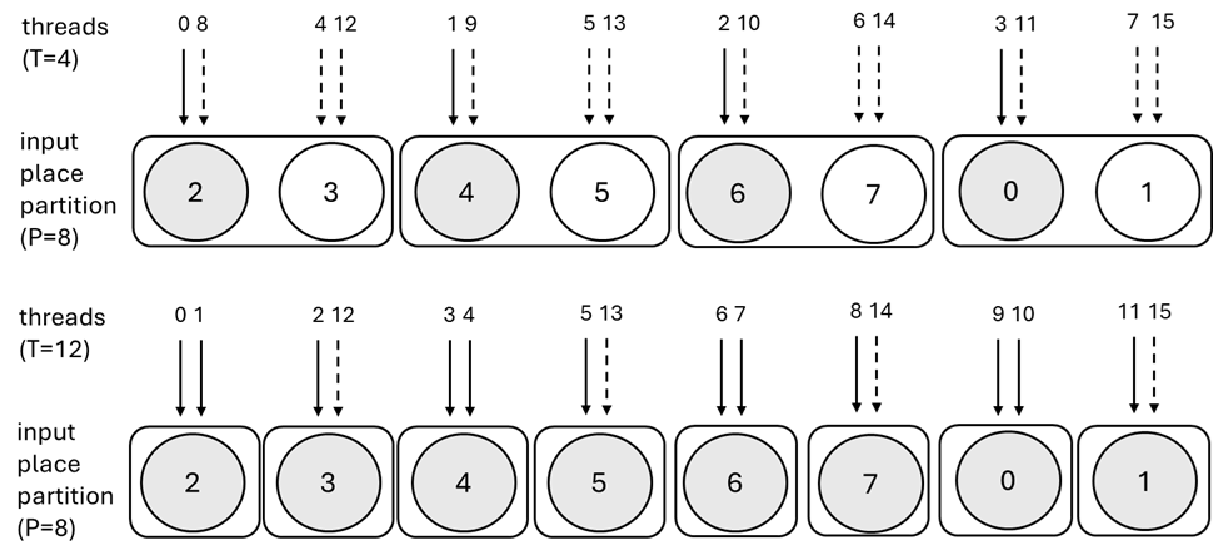
\includegraphics[width=0.7\textwidth]{figs/spread_policy}
    \caption{\kcode{spread} affinity policy}
    \label{fig:spread_policy}
\end{subfigure}

\vspace{2mm}

\begin{subfigure}[b]{0.95\textwidth}
    \centering
    \captionsetup{justification=centering}
    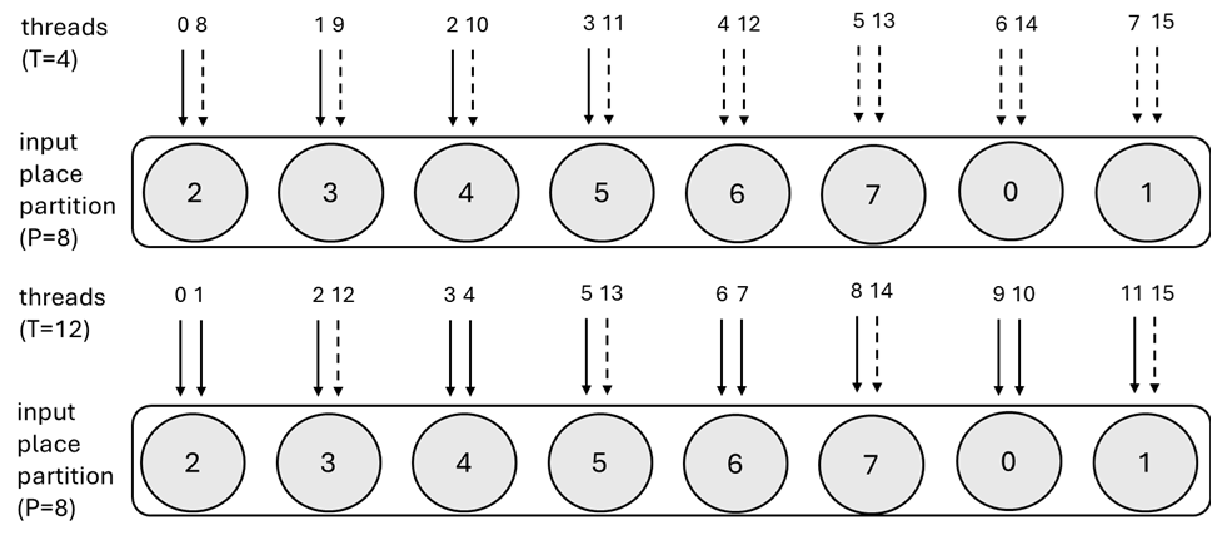
\includegraphics[width=0.7\textwidth]{figs/close_policy}
    \caption{\kcode{close} affinity policy}
    \label{fig:close_policy}
\end{subfigure}

\vspace{2mm}

\begin{subfigure}[b]{0.95\textwidth}
    \centering
    \captionsetup{justification=centering}
    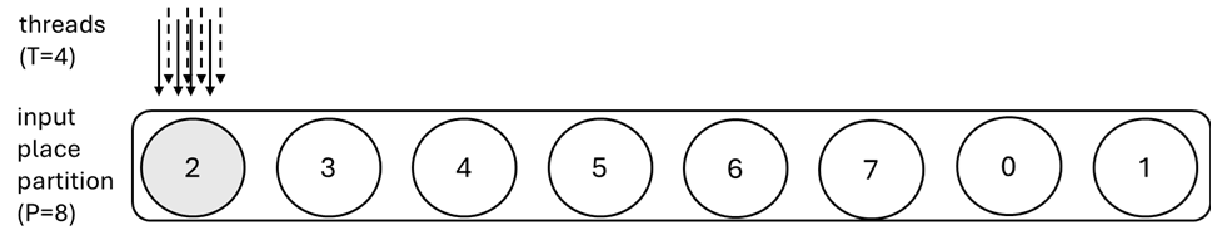
\includegraphics[width=0.7\textwidth]{figs/primary_policy}
    \caption{\kcode{primary} affinity policy}
    \label{fig:primary_policy}
\end{subfigure}

\caption{Thread Affinity Illustrations}
    \label{fig:affinity_illustrations}
\end{figure}


There are three policies:

\begin{itemize}
\item The \kcode{spread} policy divides the input place partition into
subpartitions and then distributes the threads to a place in each of the
subpartitions while setting the \plc{place-partition-var} ICV for each
thread to the subpartition to which it is distributed. This policy
can be useful for reducing resource contention between threads that
execute in the parallel region or if threads are expected to spawn
nested parallelism that is confined to their new place subpartition. 

\item The \kcode{close} policy round-robin assigns threads (one or more at a
time) to places in the input place partition. The \plc{place-partition-var}
ICV for each thread is set to the input place partition of the region.

\item The \kcode{primary} policy is used to ensure all threads are assigned to
the same place, which is the place of the encountering thread if it is bound to
a place. Again, each thread inherits the input place partition for its
\plc{place-partition-var} ICV.
\end{itemize} 

Let $T$ be the team size and $P$ be the number of places in the input place
partition. For the \kcode{spread} policy, when $T < P$ the input place
partition is subdivided into $T$ subpartitions of $\lceil P/T \rceil$ or
$\lfloor P/T \rfloor$ places, and otherwise the input place partition is
subdivided into $P$ subpartitions of one place each. The first place of each of
the subpartitions is \emph{team-eligible} for place assignment (meaning one of
the $T$ team threads can be assigned to it). For the \kcode{close} policy, each
place in the input place partition is team-eligible for place assignment.
Finally, for the \kcode{primary} policy only the place to which the primary
thread is assigned (or will be assigned as chosen by the implementation) is
team-eligible for place assignment. In Figure~\ref{fig:affinity_illustrations},
the team-eligible places are depicted as gray circles.

Let $Q$ be the number of team-eligible places in the input place partition. When
$T > Q$, the $T$ threads that comprise the team are divided into $Q$ sets of
$\lceil T/Q \rceil$ or $\lfloor T/Q \rfloor$ consecutive threads, and otherwise
they are divided into $T$ sets of one thread each. The first thread set is
assigned to the place of the primary thread if that thread is already assigned,
and otherwise the thread set is assigned to one of the $Q$ team-eligible
places. The next thread set is then assigned to the next team-eligible place,
and so on with wrap-around.

For the \kcode{spread} policy when $T > P$ or for the \kcode{close} policy,
after the $T$ threads are assigned there will be $K = P - T \bmod P$
team-eligible places with one less thread than the rest. If $K < P$, each of
the first $K$ free-agent threads that begin execution in the parallel region
will be assigned to one these places, in some order defined by the
implementation. The bottom case of Figure~\ref{fig:spread_policy} and both
cases of Figure~\ref{fig:close_policy} provide an illustration of such
assigments.

% NOTE: the round-robin assingment of additional free-agent threads may be
% relaxed in OpenMP 6.1. Keeping this for now.
Any additional free-agent threads are handled as follows. For the
\kcode{spread} policy when $T \le P$, the first free-agent thread goes to the
subpartition to which the primary thread is assigned, the next free-agent
thread goes to the next subpartition, and so on with wrap-around. Within each
subpartition, free-agent threads are round-robin assigned to the allotted
places with wrap-around, starting with the second place in the subpartition if
it has more than one place. See the top case of Figure~\ref{fig:spread_policy}
for an illustration of such assignments. For all other cases, additional
free-agent threads are round-robin assigned to team-eligible places in the
input place partition with wrap-around, starting with the place to which the
primary thread is assigned.

The following example demonstrates how to control thread affinity for a
parallel region according to an affinity policy. The machine architecture
assumed for this example is depicted in Figure~\ref{fig:mach_arch}. It consists
of two sockets, each equipped with a quad-core processor and configured to
execute two hardware threads simultaneously on each core. These examples assume
a contiguous core numbering starting from $0$, such that the hardware threads
$0$,$1$ form the first physical core.

\ifpdf
\begin{figure}[htb]
\centerline{\includegraphics[width=3.0in,keepaspectratio=true]%
{figs/proc_bind_fig.pdf}}
\caption{A machine architecture with two quad-core processors}
\label{fig:mach_arch}
\end{figure}
\fi

The following equivalent place list declarations consist of eight places (which 
we designate as p0 to p7):
\begin{boxeducode}
\kcode{export OMP_PLACES=}"{0,1},{2,3},{4,5},{6,7},{8,9},{10,11},{12,13},
{14,15}"
\end{boxeducode}
or
\begin{boxeducode}
\kcode{export OMP_PLACES=}"{0:2}:8:2"
\end{boxeducode}
or
\begin{boxeducode}
\kcode{export OMP_PLACES=}"cores"
\end{boxeducode}

\cexample[6.0]{affinity_control}{1}
\clearpage

\ffreeexample[6.0]{affinity_control}{1}

The example is simple: a \kcode{parallel} construct in which there is a call to
an external procedure \ucode{work}. By setting \kcode{OMP_NUM_THREADS} to \pout{4}
and \kcode{OMP_THREAD_LIMIT} to \pout{16}, the construct will spawn a team of size 4
and will allow for up to 12 additional free-agent threads to join in the execution
of tasks in \ucode{work}. Note that the OpenMP 6.0 specification also allows for
\kcode{OMP_NUM_THREADS} and \kcode{OMP_THREAD_LIMIT} to be set to a
\emph{numeric abstract name}. For example, setting \kcode{OMP_THREAD_LIMIT} to
\pout{"n_threads"} will set it to the number of hardware threads available on
the device, which again is 16 for the machine we are assuming.

The thread affinity policy can then be controlled via the \kcode{OMP_PROC_BIND}
environment variable. 
If \kcode{OMP_PROC_BIND} is set to
a comma separated list of \kcode{spread}, \kcode{close}, or \kcode{primary},
then each element of the list is used for each level of parallelism from left
to right. For example, setting \kcode{OMP_PROC_BIND} to \pout{"spread,close"}
will apply the \kcode{spread} affinity policy to the outer active
\kcode{parallel} region and a \kcode{close} affinity policy (operating within
an updated place partition) for an inner active \kcode{parallel} region.


\section{\kcode{proc\_bind} Clause} \label{sec:affinity}
\index{affinity!proc_bind clause@\kcode{proc_bind} clause}
\index{clauses!proc_bind@\kcode{proc_bind}} \index{proc_bind
clause@\kcode{proc_bind} clause}

The following examples demonstrate how to use the \kcode{proc_bind} clause to
control the thread binding for a team of threads in a \kcode{parallel} region.
The same machine architecture and place list from the preceding section is
assumed.

\subsection{Spread Affinity Policy} \label{subsec:affinity_spread}
\index{affinity!spread policy@\kcode{spread} policy} \index{spread
policy@\kcode{spread} policy}


The following example shows the result of the \kcode{spread} affinity policy on
the partition list when the number of threads is less than or equal to the
number of places in the parent's place partition, for the machine architecture
depicted above. Note that the threads are bound to the first place of each
subpartition.

\cexample[4.0]{affinity}{1}

\fexample[4.0]{affinity}{1}

It is unspecified on which place the primary thread is initially started. If the 
primary thread is initially started on p0, the following placement of threads will 
be applied in the parallel region:

\begin{compactitem}
\item thread 0 executes on p0 with the place partition p0,p1

\item thread 1 executes on p2 with the place partition p2,p3

\item thread 2 executes on p4 with the place partition p4,p5

\item thread 3 executes on p6 with the place partition p6,p7
\end{compactitem}


If the primary thread would initially be started on p2, the placement of threads 
and distribution of the place partition would be as follows:

\begin{compactitem}
\item thread 0 executes on p2 with the place partition p2,p3

\item thread 1 executes on p4 with the place partition p4,p5

\item thread 2 executes on p6 with the place partition p6,p7

\item thread 3 executes on p0 with the place partition p0,p1
\end{compactitem}

The following example illustrates the \kcode{spread} thread affinity policy when 
the number of threads is greater than the number of places in the parent's place 
partition.

Let \ucode{T} be the number of threads in the team, and \ucode{P} be the number of places in the 
parent's place partition. The first \ucode{T/P} threads of the team (including the primary
thread) execute on the parent's place. The next \ucode{T/P} threads execute on the next 
place in the place partition, and so on, with wrap around. 

\cexample[4.0]{affinity}{2}

\ffreeexample[4.0]{affinity}{2}

It is unspecified on which place the primary thread is initially started. If the 
primary thread is initially started on p0, the following placement of threads will 
be applied in the parallel region:

\begin{compactitem}
\item threads 0,1 execute on p0 with the place partition p0

\item threads 2,3 execute on p1 with the place partition p1

\item threads 4,5 execute on p2 with the place partition p2

\item threads 6,7 execute on p3 with the place partition p3

\item threads 8,9 execute on p4 with the place partition p4

\item threads 10,11 execute on p5 with the place partition p5

\item threads 12,13 execute on p6 with the place partition p6

\item threads 14,15 execute on p7 with the place partition p7
\end{compactitem}

If the primary thread would initially be started on p2, the placement of threads 
and distribution of the place partition would be as follows:

\begin{compactitem}
\item threads 0,1 execute on p2 with the place partition p2

\item threads 2,3 execute on p3 with the place partition p3

\item threads 4,5 execute on p4 with the place partition p4

\item threads 6,7 execute on p5 with the place partition p5

\item threads 8,9 execute on p6 with the place partition p6

\item threads 10,11 execute on p7 with the place partition p7

\item threads 12,13 execute on p0 with the place partition p0

\item threads 14,15 execute on p1 with the place partition p1
\end{compactitem}

\subsection{Close Affinity Policy}
\label{subsec:affinity_close}
\index{affinity!close policy@\kcode{close} policy}
\index{close policy@\kcode{close} policy}

The following example shows the result of the \kcode{close} affinity policy on 
the partition list when the number of threads is less than or equal to the number 
of places in parent's place partition, for the machine architecture depicted above. 
The place partition is not changed by the \kcode{close} policy.

\cexample[4.0]{affinity}{3}
\clearpage

\fexample[4.0]{affinity}{3}

It is unspecified on which place the primary thread is initially started. If the 
primary thread is initially started on p0, the following placement of threads will 
be applied in the \kcode{parallel} region:

\begin{compactitem}
\item thread 0 executes on p0 with the place partition p0-p7

\item thread 1 executes on p1 with the place partition p0-p7

\item thread 2 executes on p2 with the place partition p0-p7

\item thread 3 executes on p3 with the place partition p0-p7
\end{compactitem}

If the primary thread would initially be started on p2, the placement of threads 
and distribution of the place partition would be as follows:

\begin{compactitem}
\item thread 0 executes on p2 with the place partition p0-p7

\item thread 1 executes on p3 with the place partition p0-p7

\item thread 2 executes on p4 with the place partition p0-p7

\item thread 3 executes on p5 with the place partition p0-p7
\end{compactitem}

The following example illustrates the \kcode{close} thread affinity policy when 
the number of threads is greater than the number of places in the parent's place 
partition.

Let \ucode{T} be the number of threads in the team, and \ucode{P} be the number of places in the 
parent's place partition. The first \ucode{T/P} threads of the team (including the primary
thread) execute on the parent's place. The next \ucode{T/P} threads execute on the next 
place in the place partition, and so on, with wrap around. The place partition 
is not changed by the \kcode{close} policy.

\cexample[4.0]{affinity}{4}

\ffreeexample[4.0]{affinity}{4}

It is unspecified on which place the primary thread is initially started. If the 
primary thread is initially running on p0, the following placement of threads will 
be applied in the parallel region:

\begin{compactitem}
\item threads 0,1 execute on p0 with the place partition p0-p7

\item threads 2,3 execute on p1 with the place partition p0-p7

\item threads 4,5 execute on p2 with the place partition p0-p7

\item threads 6,7 execute on p3 with the place partition p0-p7

\item threads 8,9 execute on p4 with the place partition p0-p7

\item threads 10,11 execute on p5 with the place partition p0-p7

\item threads 12,13 execute on p6 with the place partition p0-p7

\item threads 14,15 execute on p7 with the place partition p0-p7
\end{compactitem}

If the primary thread would initially be started on p2, the placement of threads 
and distribution of the place partition would be as follows:

\begin{compactitem}
\item threads 0,1 execute on p2 with the place partition p0-p7

\item threads 2,3 execute on p3 with the place partition p0-p7

\item threads 4,5 execute on p4 with the place partition p0-p7

\item threads 6,7 execute on p5 with the place partition p0-p7

\item threads 8,9 execute on p6 with the place partition p0-p7

\item threads 10,11 execute on p7 with the place partition p0-p7

\item threads 12,13 execute on p0 with the place partition p0-p7

\item threads 14,15 execute on p1 with the place partition p0-p7
\end{compactitem}

\subsection{Primary Affinity Policy}
\label{subsec:affinity_primary}
\index{affinity!primary policy@\kcode{primary} policy}
\index{primary policy@\kcode{primary} policy}

The following example shows the result of the \kcode{primary} affinity policy on 
the partition list for the machine architecture depicted above. The place partition 
is not changed by the primary policy.

\cexample[5.1]{affinity}{5}

\fexample[5.1]{affinity}{5}

It is unspecified on which place the primary thread is initially started. If the 
primary thread is initially running on p0, the following placement of threads will 
be applied in the parallel region:

\begin{compactitem}
\item threads 0-3 execute on p0 with the place partition p0-p7
\end{compactitem}

If the primary thread would initially be started on p2, the placement of threads 
and distribution of the place partition would be as follows:

\begin{compactitem}
\item threads 0-3 execute on p2 with the place partition p0-p7
\end{compactitem}



\input{affinity/task_affinity}
\input{affinity/affinity_display}
\input{affinity/affinity_query}

